% !TEX encoding = UTF-8 Unicode 
% !TEX root = praca.tex

\chapter*{Wprowadzenie}

We współczesnym środowisku medycznym akwizycja i przetwarzanie biosygnałów,
w szczególności elektrokardiogramu (\textit{EKG}), stanowią kluczowe aspekty diagnostyki oraz
monitorowania zdrowia \cite{Serhani2020}. W świetle globalnej tendencji wzrostu 
przypadków zachorowań na przewlekłe choroby układu krążenia \cite{Gaidai2023}, 
rośnie zapotrzebowanie na tanie, efektywne i dostępne narzędzia diagnostyczne. 
Dostępność tych narzędzi, zwłaszcza w przypadku osób prywatnych oraz w warunkach słabo rozwiniętych 
systemów ochrony zdrowia, staje się poważnym wyzwaniem dla współczesnej medycyny \cite{Faruk2021}.

Przyjrzenie się obecnej sytuacji w obszarze medycyny ukazuje ograniczenia w dostępie do 
sprzętu oraz oprogramowania diagnostycznego, co jest szczególnie zauważalne w krajach rozwijających się \cite{Faruk2021}. 
W konsekwencji, potrzeba stworzenia prostych, tanich i powszechnie dostępnych narzędzi diagnostycznych, umożliwiających 
akwizycję i wstępne przetwarzanie sygnału \textit{EKG}, stała się motywacją oraz impulsem do podjęcia tematu tej pracy.

Przedstawione wyżej wyzwania podkreślają potrzebę rozwoju rozwiązań, które nie tylko zapewnią powszechny dostęp
do diagnostyki, ale również umożliwią błyskawiczną i efektywną analizę biosygnałów, wspierając tym samym szybkie 
i wczesne podejmowanie decyzji klinicznych. W ramach niniejszej pracy inżynierskiej, skoncentrowanej stworzeniu urządzenia 
oraz dedykowanego mu oprogramowania, zaproponowano prototyp taniego i dostępnego narzędzia diagnostycznego. 

Elektrokardiogram (\textit{EKG}) jest wynikiem aktywności elektrycznej serca, spowodowanej skurczem i rozkurczem tego mięśnia 
\cite{Limaye2016}. Sygnał \textit{EKG} jest funkcją mierzonego napięcia w czasie. 
Jeden cykl składający się ze skurczu i rozkurczy, reprezentowany jest przez zespoł tzw. \textit{załamków} 
oznaczonych literami \textit{P}, \textit{Q}, \textit{R}, \textit{S} i \textit{T} przedstawionymi na rys \ref{fig:pqrst}.

Zasadniczą trudnością w systemach akwizycji i przetwarzania sygnałów jest efektywna eliminacja zakłóceń (\textit{szumów}), które
znacząco utrudniają proces diagnostyczny w przypadku sygnału \textit{EKG}. Wśród nich wyróżnić można m. in. \cite{Limaye2016}: 
dryft linii izoelektrycznej (\textit{baseline wander}), 
szumy indukowane przez instalacje elektryczne w budynkach (\textit{power line interference noise}) 
czy artefakty spowodowane ruchem pacjenta. Jedną ze sprawdzonych metod eliminacji szumów są filtry cyfrowe, w tym filtry 
o skończonej odpowiedzi impulsowej \textit{FIR} (\textit{Finite Impulse Response}) \cite{Tompkins1993}.

\begin{figure}[h!]
    \centering
    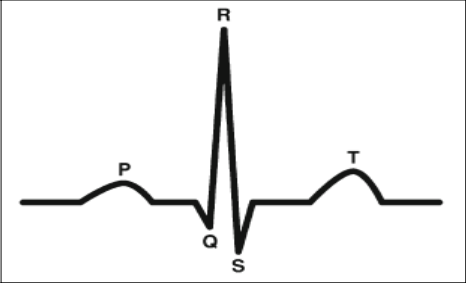
\includegraphics[scale=0.6]{pl/media/pqrst.png}
    \caption{Zespoł załamków \textit{PQRST} (\cite{Limaye2016}, fig. 1.)}
    \label{fig:pqrst}
\end{figure}

\newpage

\section*{Cel i zakres pracy}

Celem pracy było stworzenie sprzętowego oraz programowego systemu akwizycji i wstępnego przetwarzania sygnału \textit{EKG} 
mającego znamiona narzędzia diagnostycznego. W zamyśle pracy było stworzenie prototypowego systemu przeznaczonego 
do użytku prywatnego, w tym do wstępnej i samodzielnej oceny stanu mięśnia sercowego a następnie
potencjalnej konsultacji lekarskiej.  
Autor zastrzega jednak, że praca ma wymiar edukacyjny, a celem jej nie było stworzenie narzędzia diagnostycznego spełniającego 
standardy urządzenia medycznego.


Niniejsza praca opisuje projekt i realizację dwóch części:

\begin{itemize}

    \item \textbf{sprzętowej}: makieta układu elektronicznego\footnote{Przez makietę rozumiany jest prototyp urządzenia typu 
    \textit{PoC} (ang. \textit{Proof of Concept})}, zawierająca układ wzmacniacza, filtry analogowe, 
    mikrokontroler, programator sprzętowy oraz mostek \textit{USB}/\textit{UART},


    \item \textbf{programowej}: oprogramowanie sprzętowe (inaczej \textit{firmware}), aplikacja na komputery PC 
    (zwana w dalszych rozdziałach \textit{aplikacją}) oraz programy/skrypty wspomagające projektowanie filtrów cyfrowych 
    (zwane krócej \textit{skryptami}).

\end{itemize}

Część sprzętowa odpowiada za wstępne wzmocnienie i analogową filtrację sygnału \textit{EKG} 
oraz umożliwienie komunikacji z komputerem PC na którym zainstalowana jest wspomniana aplikacja. 


Oprogramowanie sprzętowe (na układ mikrokontrolera makiety sprzętowej) umożliwiło obsługę przetwornika analogowo/cyfrowego,
implementację filtrów cyfrowych oraz implementację protokołu oraz obsługę interfejsu do komunikacji z komputerem PC.
Aplikacja na komputery PC została stworzona w celu podglądu sygnału oraz jego zapisu w czasie rzeczywistym.

\newpage

\section*{Użyty sprzęt oraz technologie}

Ze względu prototypowy charakter pracy, część sprzętowa zrealizowana została jako makieta w oparciu o gotowe
płytki drukowane z układami elektronicznymi. W skład części sprzętowej wchodzą następujące elementy, szczegółowiej
opisane w rozdziale 2:

\begin{itemize}

    \item płytka z układem \textbf{AD8232} \cite{AD8232BS} \cite{AD8232ds}: zawiera filtry analogowe oraz układ wzmacniaczy,


    \item płytka z mikrokontrolerem \textbf{STM32F411} oraz programatorem \textbf{STLink v2} \cite{STM32F4DS} \cite{NUCLEO}: 
    zawiera mikrokontroler z mikroprocesorem \textit{ARM Cortex M4} oraz układami peryferyjnymi takimi jak: 
    przetwornik analogowo/cyfrowy, liczniki czy kontroler \textit{DMA} (\textit{Direct Memory Access}),
    

    \item przewody połączeniowe, w tym przewód \textit{USB} do połączenia makiety z komputerem PC.


\end{itemize}

W części programowej użyto następujących języków, bibliotek i narzędzi:

\begin{itemize}

    \item \textbf{język C} (standard \textit{C11}): język kompilowany użyty w implementacji oprogramowania sprzętowego,

    \item \textbf{język C++} (standard \textit{C++20}): język kompilowany użyty w implementacji 
    protokołu komunikacyjnego oraz aplikacji,

    \item \textbf{ARM GNU Embedded Toolchain} \footnote{\url{https://developer.arm.com/downloads/-/gnu-rm}}: zestaw narzędzi, w tym
    kompilatorów języków \textit{C} i \textit{C++} oraz \textit{assemblera} dla mikroprocesorów \textit{ARM Cortex-M},

    \item \textbf{biblioteka STM32HAL} \cite{STM32HAL}: biblioteka dostarczająca warstwę abstrakcji dla mikroprocesora 
    oraz układów peryferyjnych mikrokontrolera \textit{STM32F411}.

    \item \textbf{SDL2} \cite{SDL2}: biblioteka umożliwiająca renderowanie rastrowej grafiki dwuwymiarowej zastosowana
    do implementacji wykresu sygnału w aplikacji,

    \item \textbf{standardowe biblioteki języków C i C++ na system GNU/Linux} \cite{GLIBC238}: biblioteki użyte do 
    implementacji komunikacji międzyprocesowej, wielowątkowości oraz niektórych struktur danych w aplikacji,

    \item \textbf{język Python 3} \footnote{\url{https://www.python.org/}}: język skryptowy użyty do napisania 
    skryptów obliczeniowych i pomocniczych w projektowaniu filtrów cyfrowych,
   
    \item \textbf{CMake} \footnote{\url{https://cmake.org/}} \textbf{oraz GNU Make} 
    \footnote{\url{https://www.gnu.org/software/make/}}: systemy automatyzujące 
    kompilację i linkowanie aplikacji w \textit{C} i \textit{C++}.

\end{itemize}

